\documentclass[10pt,xcolor=dvipsnames]{beamer}
\usepackage{graphicx}
\usepackage{multimedia}
\usepackage{epsf,amsmath,amssymb,amsfonts}
\usepackage{tikz}
\usetikzlibrary{decorations}
\usetheme{CambridgeUS}

%---------------------------------------------------------------------------
%
%          USER DEFINED MACROS
%
%\mathsurround = 2pt

\def \ds          {\displaystyle}
\def \rmd         {{\rm d}}
\def \be          {{\bf e}}
\def \bF          {{\bf F}}
\def \bI          {{\bf I}}
\def \bn          {{\bf n}}
\def \bff         {{\bf f}}
\def \bdf         {{\bf df}}
\def \bdT         {{\bf dT}}
\def \bT          {{\bf T}}
\def \cT          {{\cal T}}
\def \bU          {{\bf U}}
\def \bu          {{\bf u}}
\def \bv          {{\bf v}}
\def \bV          {{\bf V}}
\def \bX          {{\bf X}}
\def \by          {{\bf y}}
\def \bY          {{\bf Y}}
\def \bz          {{\bf z}}
\def \bZ          {{\bf Z}}
\def \bW          {{\bf W}}
\def \bZt         {{\bf \widetilde Z}}
\def \bzi         {{\bz}_i}
\def \bzs         {{\bz}^*}
\def \bzis        {{\bz}_i^*}
\def \bzin        {\{\bzi\}_{i=1}^k}
\def \cf          {{\cal F}}
\def \cg          {{\cal G}}
\def \ch          {{\cal H}}
\def \vi          {{V_i}}
\def \vin         {\{\vi\}_{i=1}^k}
\def \Babs        {{\Big|}}
\def \Bl          {{\Big(}}
\def \Br          {{\Big)}}
\def \Bleft       {{\Big[}}
\def \Bright      {{\Big]}}
\def \p           {\partial}
\def \R           {{\mathbb R}}
\def \N           {{\mathbb N}}
\def\y            {{\bf y}}
\def \tN          {{\widetilde{N}}}
\def \tD          {{\widetilde{D}}}

\def \proofnote #1{\footnote{{\bf Note: #1}}}
\def \norm      #1{\left\|\,#1\,\right\|}
\def \set       #1{\left\{\,#1\,\right\}}
\def \tr          {^T}
\def \IhH         {I_h^H}
\def \IhHb        {{\hat I}_h^H}
\def \IHh         {I_H^h}
\def \vbar        {\bar v}
\def \zhbar       {\bar z_h}
\def \zHbar       {\bar z_H}
\def \zhplus      {z_h^+}
\def \zHplus      {z_H^+}

\renewcommand{\theequation}{\thesection.\arabic{equation}}

\newtheorem{alg}{Algorithm}[section]
\newtheorem{thm}{Theorem}[section]
\newtheorem{lem}[thm]{Lemma}
\newtheorem{cor}[thm]{Corollary}
\newtheorem{pro}{Proposition}[section]
\newtheorem{defn}{Definition}[section]
\newtheorem{asp}{Assumption}[section]
\newtheorem{rmk}{Remark}[section]

%\def \Rblack#1{\,\hbox{R \kern-1.2em I
%    \kern.275em $^{#1}$}}
%\def \bG{{\bf G}}
%\def \bt{{\bf t}}
%\def \bzj{{\bz}_j}
%\def \bY{{\bf Y}}
%\def \byi{{\by}_i}
%\def \byj{{\by}_j}
%\def \byim{\{\byi\}_{i=1}^m}
%\def \bx{{\bf x}} 


\author[Zichao Di]{Zichao Di}


\title{Introduction of Multigrid}
\date{\today}
\setbeamertemplate{navigation symbols}{}
\begin{document}
\frame{\titlepage}
%%%%%%%%%%%%%%%%%%%%%%%%%%%%%%%%%%%%%%


\section{Outline}
\subsection{Outline}
\frame{
\frametitle{Outline}
\begin{itemize}
\item{\em {\color{blue}Model Problems}}

\item  {\color{blue}Development of Multigrid}
\begin{itemize}
\item Coarse-grid correction
\item Nested Iteration
\item Restriction and Interpolation
\item Standard cycles: MV, FMG
\end{itemize}



\item {\color{blue}Summary and discussion}
\end{itemize}
}
%%%%%%%%%%%%%%%%%%%%%%%%%%%%%%%%%


\section{Multigrid}
\subsection{Introduction}
\frame{
\frametitle{{\color{Blue}Model Problems}}
\begin{columns}
\column{3in}
\begin{itemize}
\item{\em {\color{blue}One-dimensional boundary value problem:}}
$$
-u''(x)+\sigma u(x)=f(x)\quad \quad \quad 0<x<1, \quad \sigma>0$$
$$u(0)=u(1)=0$$
\item {\color{blue}Grid:} $h=\frac{1}{N},\quad \quad x_{i}=ih,\quad \quad i=0,1,\dots, N$\\

 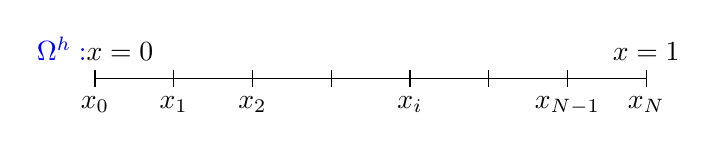
\begin{tikzpicture}
\draw (0,0) -- (1,0);
\draw (1,0) -- (2,0);
\draw (2,0) -- (3,0);
\draw (3,0) -- (4,0);
\draw (4,0) -- (5,0);
\draw (5,0) -- (6,0);
\draw (6,0) -- (7,0);
\foreach \x in {0,1,2,3,4,5,6,7}
\draw (\x cm,3pt) -- (\x cm,-3pt);
\draw (0,0) node[below=3pt] {$ x_0 $} node[above=3pt] {${\color{blue}\Omega^{h}: }x=0  $};
\draw (1,0) node[below=3pt] {$ x_1 $} node[above=3pt] {$  $};
\draw (2,0) node[below=3pt] {$ x_2 $} node[above=3pt] {$  $};
\draw (3,0) node[below=3pt] {$  $} node[above=3pt] {$  $};
\draw (4,0) node[below=3pt] {$  x_i$} node[above=3pt] {$  $};
\draw (5,0) node[below=3pt] {$  $} node[above=3pt] {$  $};
\draw (6,0) node[below=3pt] {$ x_{N-1} $} node[above=3pt] {$  $};
\draw (7,0) node[below=3pt] {$ x_N $} node[above=3pt] {$ x=1 $};
\end{tikzpicture}

\item Let $v_i\approx u(x_i)$ and $f_i\approx f(x_i)$ for $i=0,1,\dots,N$
\end{itemize}
\end{columns} 
}
 

\frame{
\frametitle{\centering{We approximate the equation with a finite difference scheme}}
\begin{itemize}
\item  We approximate the BVP
{\color{blue}
$$-u''(x)+\sigma u(x)=f(x)\quad \quad \quad 0<x<1, \quad \sigma>0$$
$$u(0)=u(1)=0$$}
with the finite difference scheme:{\color{blue}
$$\frac{-v_{i-1}+2v_{i}-v_{i+1}}{h^{2}}+\sigma v_{i}=f_{i},  i=1,2,\dots, N-1$$
$$v_{0}=v_{N}=0$$}

\end{itemize}
}

\frame{
\frametitle{The discrete model problem}
\begin{itemize}
\item Letting $v={v_1,v_2,\dots,v_{N-1}}^{T}$ and $$f=(f_1,f_2,\dots,f_{N-1})^{T}$$
we obtain the matrix equation $Av=f$ where $A$ is $(N-1)x(N-1)$, symmetric, positive definite, and 
$$
A=\frac{1}{h^{2}}\left( \begin{array}{cccccc}
2+\sigma h^{2}& -1 &  & & &  \\
-1 & 2+\sigma h^{2} &-1 & & &\\
 & -1& 2+\sigma h^{2}& -1 & & \\
& & &\dots & & \\
& &  & -1 & 2+\sigma h^{2}& -1\\
& & &  & -1& 2+\sigma h^{2}\\
\end{array} \right)$$
$$ v=\left(\begin{array}{c}
v_1\\
v_2\\
v_3\\
\dots\\
v_{N-2}\\
v_{N-1}\end{array}\right),\quad
 f=\left(\begin{array}{c}
f_1\\
f_2\\
f_3\\
\dots\\
f_{N-2}\\
f_{N-1}\end{array}\right)
$$
\end{itemize}
}


\frame{
\frametitle{Solution Methods}

\begin{itemize}
\item {\color{blue}Direct}
\begin{itemize}
\item Gaussian elimination
\item Factorization
\end{itemize}
\item {\color{blue}Iterative}
\begin{itemize}
\item Let $A=(D-L-U)$ where $D$ is diagonal and $L$ and $U$ are the strictly lower and upper parts of $A$
\item Jacobi
\begin{itemize}
\item Let $R_{J}=D^{-1}(L+U)$, then the iteration is :\color{blue} $$v^{new}=R_{J} v^{old}+D^{-1}f$$
\end{itemize}
\item Gauss-Seidel  (1D)
\begin{itemize}
\item Let $R_{G}=(D-L)^{-1}U$, then the iteration is: \color{blue} $$v^{new}=R_{G} v^{old}+(D-L)^{-1}f$$
\end{itemize}
\item Conjugate Gradient, etc.
\end{itemize}
\end{itemize} 
}


\frame{
\frametitle{Analysis of stationary iterations}
\begin{itemize}
\item Let $v^{new}=Rv^{old}+g$. The exact solution is unchanged by the iteration, i.e., $u=Ru+g$
\item Subtracting, we have the error propagation: $$e^{new}=Re^{old}$$
\item With $e^{0}$ be the initial error, after $ith$ iteration, we have $$e^{n}=R^{n}e^{0}$$
\end{itemize}

}

\frame{
\frametitle{Fundamental theorem of iteration}
\begin{itemize}
\item $R$ is convergent ($R^{n}\rightarrow 0$ as $n\rightarrow \infty$) if and only if $\rho(R)<1$, where $\rho(R)=max\{| \lambda_{1}|, |\lambda_{2}|,\dots,|\lambda_{N}|\}$
\item Therefore, for any initial vector $v^{0}$, wer see that $e^{n}\rightarrow 0$ as $n\rightarrow \infty$ if and only if $\rho(R)<1$
\item $\rho(R)<1$ assures the convergence of the iteration given by $R$ and $\rho(R)$ is called the {\color{green}convergence factor} for the iteration.
\item Since $\frac{\|e^{M}\|}{\|e^{0}\|}\leq \|R^{M}\|$, so we use $(\frac{\|e^{M}\|}{\|e^{0}\|})^{\frac{1}{M}}$ to measure the convergence factor
\end{itemize}
}

\frame{
\frametitle{First observation toward multigrid}
\begin{itemize}
\item Many relaxation schemes have the smoothing property, where oscillatory modes of the error are eliminated effectively, but smooth modes are damped very slowly.
\item This might seem like a limitation, but by using coarse grids we can use the smoothing property to good advantage.
 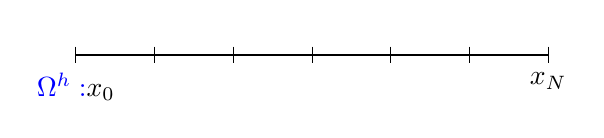
\begin{tikzpicture}
\draw (0,0) -- (1,0);
\draw (1,0) -- (2,0);
\draw (2,0) -- (3,0);
\draw (3,0) -- (4,0);
\draw (4,0) -- (5,0);
\draw (5,0) -- (6,0);
\foreach \x in {0,1,2,3,4,5,6}
\draw (\x cm,3pt) -- (\x cm,-3pt);
\draw (0,0) node[below=3pt] {${\color{blue}\Omega^{h}: } x_0 $} node[above=3pt] {$ $};
\draw (6,0) node[below=3pt] {$ x_N $} node[above=3pt] {$  $};

\end{tikzpicture}

 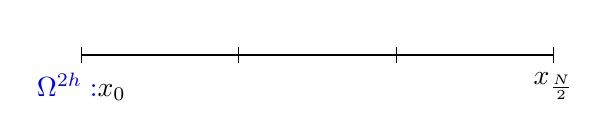
\begin{tikzpicture}
\draw (0,0) -- (2,0);
\draw (2,0) -- (4,0);
\draw (4,0) -- (6,0);
\foreach \x in {0,2,4,6}
\draw (\x cm,3pt) -- (\x cm,-3pt);
\draw (0,0) node[below=3pt] {${\color{blue}\Omega^{2h}: } x_0 $} node[above=3pt] {$ $};
\draw (6,0) node[below=3pt] {$ x_{\frac{N}{2}} $} node[above=3pt] {$$};

\end{tikzpicture}


\item Why use coarse grids ?

\end{itemize}
}

\frame{
\frametitle{Reason $\# 1$ for using coarse grids: \color{red}Nested Iteration}
\begin{itemize}
\item Coarse grids can be used to compute an improved initial guess for the fine-grid relaxation. This is advantageous because:
\begin{itemize}
\item Relaxation on the coarse-grid is much cheaper (1/2 as many points in 1D, 1/4 in 2D, 1/8 in 3D)
\item Relaxation on the coarse grid has a marginally better convergence factor, for example
  $$1-O(4h^{2})\quad \quad instead\quad  of \quad \quad 1-O(h^{2})$$
\end{itemize}
\end{itemize}
}

\frame {
\frametitle{Reason $\#2$ for using a coarse grid: smooth error is (relatively) more oscillatory there!}
\begin{itemize}
\item A smooth function:\\

\centering
 \includegraphics[width=1.5in]{finesin.jpg}

\item Can be represented by liner interpolation from a coarser grid:
\centering
 \includegraphics[width=1.5in]{coarsin.jpg}
\end{itemize}
}

\frame{
\frametitle{Second observation toward multigrid:}
\begin{itemize}
\item Recall the residual correction idea: Let $v$ be an approximation to the solution of $Au=f$, where the residual $r=f-Av$. The the error $e=u-v$ satisfies $Ae=r$.
\item After relaxing on $Au=f$ on the fine grid, the error will be smooth. On the coarse grid, however, this error appears more oscillatory, and relaxation will be more effective
\item Therefore we go to a coarse grid and relax on the residual equation $Ae=r$, with an initial guess of $e=0$.
\end{itemize}
}

\frame{
\frametitle{{\color{red}Idea!} Coarse-grid correction}
\begin{itemize}
\item {\color{blue}Relax} on $Au=f $ on $\Omega^{h}$ to obtain an approximation $v^{h}$
\item {\color{blue}Compute} $r=f-Av^{h}$
\item {\color{blue}Relax} on $Ae=r$ on $\Omega^{2h}$ to obtain an approximation to the error, $e^{2h}$
\item {\color{blue}Correct} the approximation $v^{h}\leftarrow v^{h}+e^{2h}$
\item Clearly, we need methods for the mappings $\Omega^{h}\rightarrow \Omega^{2h}$ and $\Omega^{2h}\rightarrow \Omega^{h}$
\end{itemize}
}

\frame{
\frametitle{1D Interpolation (Prolongation)}
\begin{itemize}
\item Mapping from the coarse grid to the fine grid:
{\color{blue}$$I_{2h}^{h}: \Omega^{2h}\rightarrow \Omega^{h}$$}
\item Let $v^{h},\quad v^{2h}$ be defined on $\Omega^{h},\quad \Omega^{2h}$. Then {\color{blue}$$I_{2h}^{h}v^{2h}=v^{h}$$}

where {\color{blue}$$\{\begin{array}{c}
v_{2i}^{h}=v_{i}^{2h}\\
v_{2i+1}^{h}=\frac{1}{2}(v_{i}^{2h}+v_{i+1}^{2h}) \end{array} $$} for $0\leq i\leq \frac{N}{2}-1$
\end{itemize}
}

\frame{
\frametitle{The prolongation operator (1D)}
\begin{itemize}
\item We may regard {\color{blue}$I_{2h}^{h}$} as a linear operator from $R^{N/2-1}\rightarrow  R^{N-1}$
\item e.g., for N=8, {\color{blue}$$\left( \begin{array}{ccc}
1/2 & & \\
1 & & \\
1/2 &1/2 & \\
 & 1 & \\
& 1/2 & 1/2 \\
&      &  1\\
&    &  1/2
\end{array}\right)_{7x3}
\left(\begin{array}{c}
v_{1}^{2h}\\
v_{2}^{2h}\\
v_{3}^{2h}\end{array}\right) _{3x1}=
\left(\begin{array}{c}
v_{1}^{h}\\
v_{2}^{h}\\
v_{3}^{h}\\
v_{4}^{h}\\
v_{5}^{h}\\
v_{6}^{h}\\
v_{7}^{h}\\ \end{array}\right)_{7x1} $$}
\item {\color{blue}$I_{2h}^{h}$} has full rank, and thus null space $\{\emptyset\}$
\end{itemize}
}

\frame{
\frametitle{How well does $v^{2h}$ approximate $u$}
\begin{itemize}
\item If the exact solution $u$ of error equation is smooth,  a coarse-grid interpolant of $v^{2h}$ may do very well.
\item If $u$ is oscillatory, a coarse-grid interpolant of $v^{2h}$ may {\color{red}not} work well.
\item Therefore, nested iteration is most effective when the error is smooth!
\end{itemize}
}

\frame{
\frametitle{1D Restriction by full-weighting}
\begin{itemize}
\item Mapping from the fine grid to the coarse grid:
$$I_{h}^{2h}: \Omega^{h}\rightarrow \Omega^{2h}$$
\item Let $v^{h},v^{2h}$ be defined on $\Omega^{h},\Omega^{2h}$. Then {\color{blue}$$I_{h}^{2h}v^{h}=v^{2h}$$} where {\color{blue}$v_{i}^{2h}=\frac{1}{4}(v_{2i-1}^{h}+2v_{2i}^{h}+v_{2i+1}^{h})$}
\item Regard $I_{h}^{2h}$ as a linear operator from $R^{N-1}\rightarrow R^{N/2-1}$
\item e.g., for $N=8,$
{\color{blue}$$\left(\begin{array}{ccccccc}
1/4 & 1/2 & 1/4 &  & & & \\
&  & 1/4 &1/2  &1/4 & & \\
 &  & &  & 1/4&1/2 &1/4 \\ \end{array}\right) 
\left(\begin{array}{c}
v_{1}^{h}\\
v_{2}^{h}\\
v_{3}^{h}\\
v_{4}^{h}\\
v_{5}^{h}\\
v_{6}^{h}\\
v_{7}^{h}\\ \end{array}\right)=\left(\begin{array}{c}
v_{1}^{2h}\\
v_{2}^{2h}\\
v_{3}^{2h}\end{array}\right)$$}

\end{itemize}
}


\frame{
\frametitle{Coarse Grid Correction Scheme (V-cycle)}
\begin{enumerate}
\item {\color{blue}Relax} $\alpha_1$ times on $A^{h}u^{h}=f^{h}$ on $\Omega^{h}$ with arbitrary initial guess $v_{h}$.
\item  {\color{blue}Compute} $r^{h}=f^{h}-A^{h}v^{h}$
\item  {\color{blue}Compute} $r^{2h}=I_{h}^{2h}r^{h}$
\item  {\color{blue}Solve} $A^{2h}e^{2h}=r^{2h}$ on $\Omega^{2h}$
\item  {\color{blue}Correct fine-grid solution} $v^{h}\leftarrow v^{h}+I_{2h}^{h}e^{2h}$
\item  {\color{blue}Relax} $\alpha_2$ times on $A^{h}u^{h}=f^{h}$ on $\Omega^{h}$ with initial guess $v^{h}$
\end{enumerate}
}

\frame{
\frametitle{Building $A^{2h}$}
\begin{itemize}
\item{\color{blue} Assume that $e^{h}\in Range(I_{2h}^{h})$. Then the residual equation can be written} $$r^{h}=A^{h}e^{h}=A^{h}I_{2h}^{h}u^{2h}$$ 
\item {\color{blue}Then the residual equation on the coarse grid is:} $$I_{h}^{2h}A^{h}I_{2h}^{h}u^{2h}=I_{h}^{2h}r^{h}$$
\item {\color{blue} Therefore,we identify the coarse-grid operator} $A^{2h}$ as $$A^{2h}=I_{h}^{2h}A^{h}I_{2h}^{h}$$.
\item {\color{blue} It turns out that  the $ith$ row of $A^{2h}$ is }$\frac{1}{(2h)^{2}}[-1 \quad 2 \quad -1]$ {\color{blue} which is the $\Omega^{2h}$ version of $A^{h}$}
\end{itemize}
}

\frame{
\frametitle{The variational properties}
\begin{itemize}
\item Recall that for the 1D examples, linear interpolation and full-weighting are related by : $$I_{2h}^{h}=2(I_{h}^{2h})^{T}$$ 
\item The definition for $A^{2h}$ that resulted from the
foregoing line of reasoning is useful for both
theoretical and practical reasons. Together with
the commonly used relationship between
restriction and prolongation we have the following
“variational properties”:
\item A commonly used, and highly useful, requirement is that $I_{2h}^{h}=c(I_{h}^{2h})^{T}$ for $c\in R$
\end{itemize}
}







\section{Summary}
\frame{
\frametitle{Summary and Discussion}
\begin{itemize}
\item Multigrid has been proven on a wide variety of problems, especially elliptic PDEs, but has also found application among parabolic & hyperbolic PDEs, integral equations, evolution problems, geodesic
problems, etc.
\item With the right setup, multigrid is frequently an
optimal solver
\item Multigrid is of great interest because it is one of the
very few scalable algorithms, and can be parallelized
readily and efficiently!
\end{itemize}
}

\end{document}

